\documentclass[12pt, oneside]{article}
\usepackage[letterpaper, margin=1.2in, headsep=0.7in]{geometry}
\usepackage[english]{babel}
\usepackage[utf8]{inputenc}
\usepackage{amsmath}
\usepackage{amsfonts}
\usepackage{amssymb}
\usepackage{tikz}
\usepackage{venndiagram}

\usepackage{fancyhdr}
\pagestyle{fancy}
\fancyhf{}
\rhead{Name: \hspace{.75in} }
\lhead{BECA / Dr. Huson / Algebra 2 \\* 9 February 2018 \\* Test: Probability \& review topics\\*
Open book, open notebook}

\renewcommand{\headrulewidth}{0pt}

\title{Worksheet and test template}
\author{Chris Huson}
\date{February 2018}

\begin{document}

\begin{enumerate}

\item For each Venn diagram, write an expression representing the shaded area.
\begin{enumerate}
    \item For example, for this diagram \\*
    %\\*
    \begin{venndiagram2sets}
        \fillACapB
    \end{venndiagram2sets}
    Expression:     $A \cap B$%\\*
    \item %\\*[15pt]
    \begin{venndiagram2sets}
        \fillA
        \fillB
    \end{venndiagram2sets}
    Expression: %\\*
    \item %\\*[15pt]
    \begin{venndiagram2sets}
    \fillANotB
    \end{venndiagram2sets}
    Expression: %\\*
    \item %\*[15pt]
    \begin{venndiagram3sets}
    \fillB
    \fillACapC
    \end{venndiagram3sets}
    Expression: %\\*
\end{enumerate}

\item Using a calculator, find how many sets of four elements can be selected from a set of 15, when order does not matter, i.e. $_{15}\mathrm C_4$. \\*[20pt]

\item On May 5th, 20 horses will compete in the Kentucky Derby, ``the most exciting two minutes in sports."  Among the twenty horses, how many possible finishes of first and second place are possible?

\newpage
\item Given: The universal set is $U = \{a, b, c, d, e, f, g, h, i, j\}$\\*
\qquad $A = \{e, f, g, h, i\}$
\qquad $B = \{a, e, i\}$
\begin{enumerate}
    \item What is $n(U)$?\\*[10pt]
    \item What is $A \cup B$?\\*[10pt]
    \item What is $A \cap B$?\\*[10pt]
    \item What is $A^\prime $?\\*[10pt]
\end{enumerate}

\item A survey question has three possible responses, $A$, $B$, and $C$. Among 100 surveys, the frequency of the answers collected were as follows: $n(A)=30, n(B)=55, \text{ and } n(C)=15$. 
\begin{enumerate}
    \item If a survey is selected at random, what this the probability the response was $B$?\\*[15pt]
    \item What is the probability a survey selected at random was an answer other than $C$?\\*[15pt]
\end{enumerate}

\item The events $A$ and $B$ are mutually exclusive with $\mathrm P(A)=0.4$ and $\mathrm P(B)=0.3$. What is $\mathrm P(A \cap B)$?\\*[20pt]

\item The events $A$ and $B$ are independent with $\mathrm P(A)=0.5$ and $\mathrm P(B)=0.4$. Answer the two questions and sketch a Venn diagram representing the situation, labeling each region of the graph with the appropriate probability.
\begin{enumerate}
    \item What is $\mathrm P(A \cap B)$?\\*[20pt]
    \item What is $\mathrm P(A \cup B)$?\\*[20pt]
\end{enumerate}


\newpage
\item The universal set $U$ is defined as the set of positive integers less than 13. The subsets $A$ and $B$ are defined as follows: \\*
\qquad $A =$ \{integers that are multiples of 3\}\\*
\qquad $B =$ \{prime numbers\} \\* [5pt] 
(note: Prime numbers have only themselves and one as factors. One is not considered a prime.)
\begin{enumerate}
    \item List the members of $A$\\*[20pt]
    \item List the members of $B$\\*[20pt]
    \item Place the elements of $A$ and $B$ in the appropriate regions in the Venn diagram below.\\*[5pt]
        \begin{venndiagram2sets}[tikzoptions={scale=2.5}]
        \end{venndiagram2sets}U\\*
    \item List the items in the set $(A \cup B)^\prime $\\*[20pt]
    \item If an element is selected at random, what is the probability that it is a member of the set $A \cap B$?
\end{enumerate}

\newpage
Simplify by collecting like terms.

\item $x^2+3x -5 -2x^2-3x+5$\\*[60pt]
\item $5(z^2-2z +1) -2(z^2-5z-4)$\\*[60pt]


Solve for the value of $x$.
\item   $-12=x-4x$\\*[70pt]
\item   $\frac{1}{2}(2x-8)=-3x$\\*[60pt]


What is the slope and $y$-intercept of each equation? 
\item   $y=\frac{1}{2}x-3$\\*[20pt]
\item   $x-2y=6$\\*[40pt]

\newpage
Use pencil for graphs. Label each function with its name or equation. 
\item Given the function $f(x)=\frac{2}{3}x-4$. 
\begin{enumerate}
    \item Write down the $y$-intercept.\\*[10pt]
    \item Write down the slope of $f(x)$.\\*[10pt]
    \item Draw the function $f(x)$ on the graph below.
    \item Mark and label the point $P (3, 2)$ on the graph.
    \item A second line, $g(x)$, is parallel to $f(x)$ and passes through point $P$. Plot $g(x)$ on the graph.
    \item What is the $y$-intercept of $g(x)$?\\*[10pt]
\end{enumerate}

\begin{figure}[!ht]
    \centering
    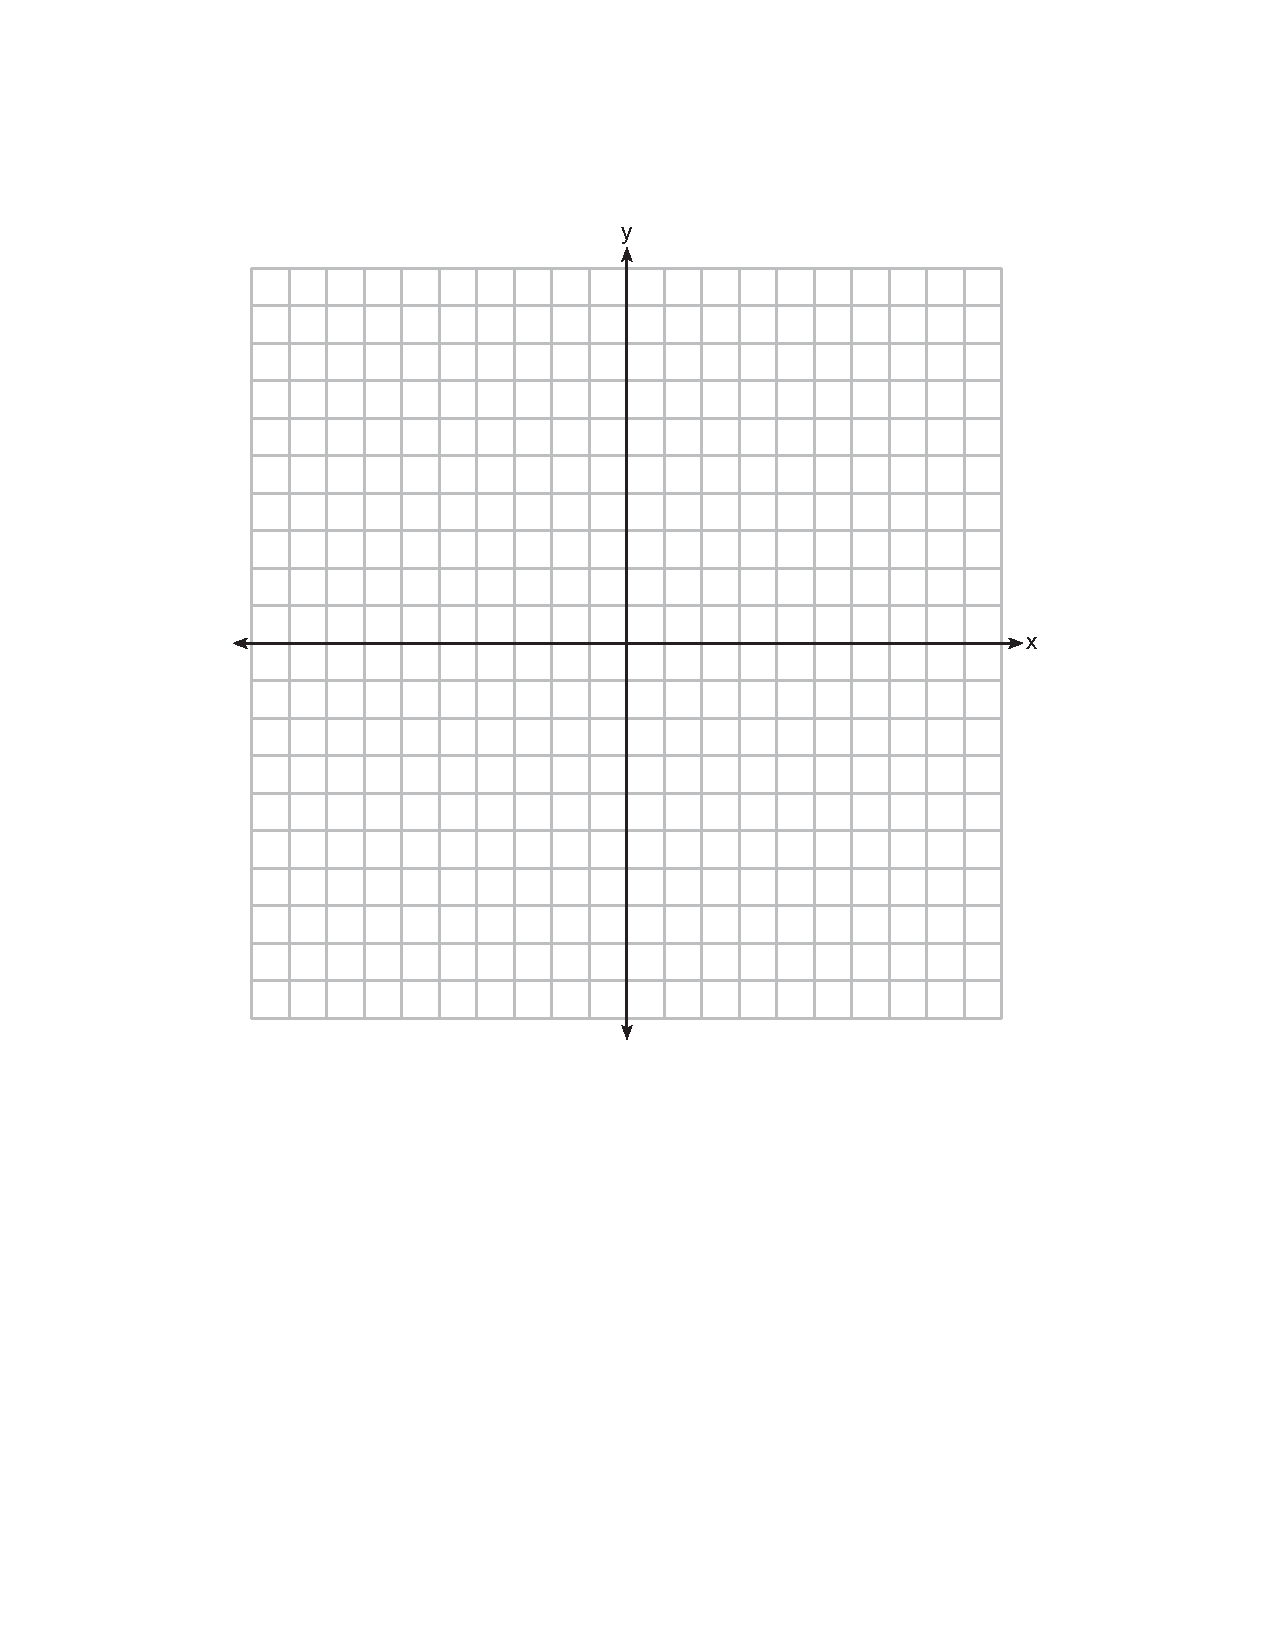
\includegraphics[width=0.75\textwidth]{regents-grid.pdf}
\end{figure}

\newpage

\item Explain why the radical $\sqrt[3]{27}$ is equivalent to $9^{\frac{1}{2}}$, an expression with a rational exponent.\\*[60pt]

\item Solve the system of equations by graphing. Select a point in the solution set and label it on the graph as ordered pair.
\[x+2y \geq 6\]
\[y < 3x-6\]

\begin{figure}[!ht]
    \centering
    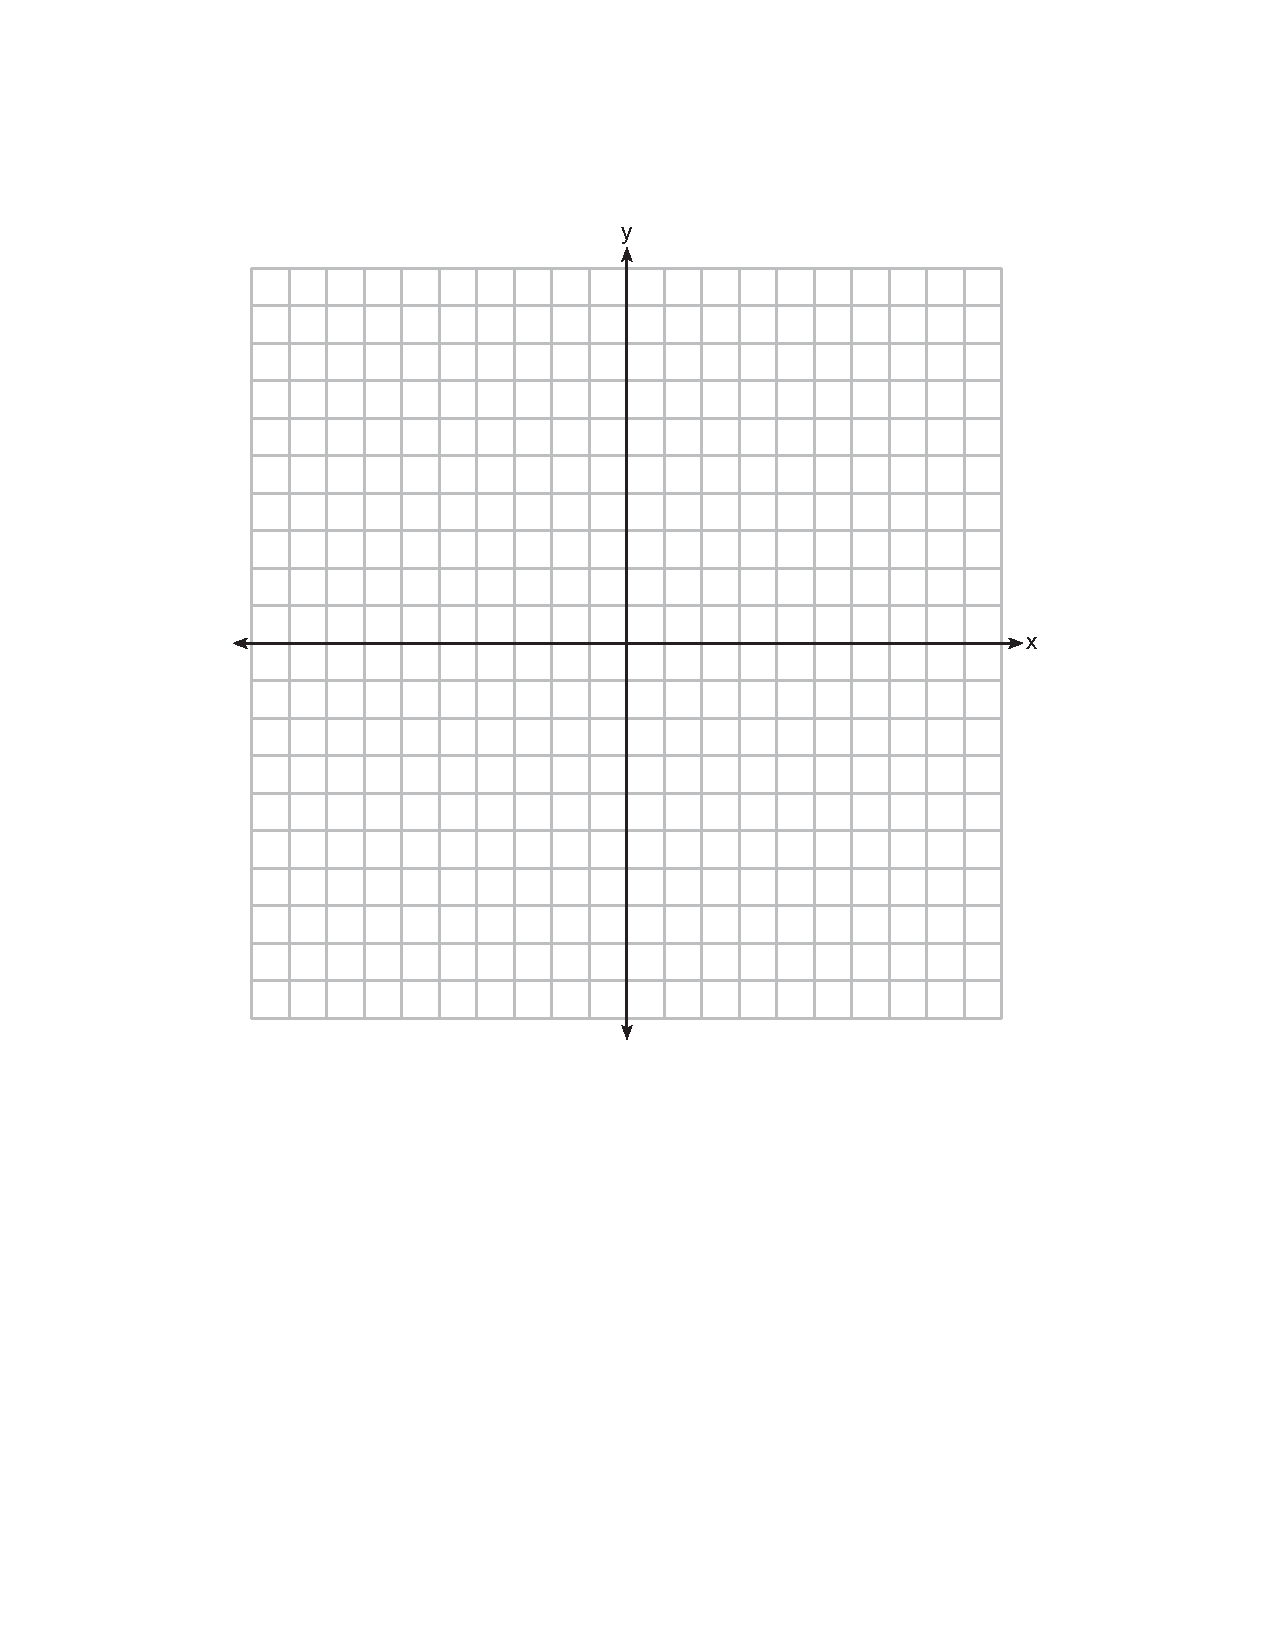
\includegraphics[width=0.65\textwidth]{regents-grid.pdf}
\end{figure}

Solve the system algebraically.
\item
$2x-y=13$\\*
$3x+y=-3$

\end{enumerate}

\end{document}
